% answers.tex —— 2009 年·普通高等学校招生考试·湖北卷·文科 · 参考答案与详细解析片段
% 由 tools/generate_projects.py 依来源总账自 2009/2009_数学真题_湖北文_试题.md + 2009/2009_数学真题_湖北文_解析正文.md + 2009/2009_数学真题_湖北文_答案要点.md 生成，勿手改（改源 MD 后重跑）


\begin{gktip}
固定候选 PDF 仅含题面，无答案、解析和评分标准，原页亦未标分值；以下为非官方编者独立推导，官方答案字段为空。分数、根号、上下标与六幅图均以 600 dpi 原页复核。原页第 10 题「性状」「成为」「及时」三处为排印问题（应为「形状」「称为」「既是」），解析按更正后的语义理解，答案不受影响。
\end{gktip}

\begin{answer}
\gksolhead{1}{}

\textbf{题目}：

若向量 $\boldsymbol a=(1,1)$，$\boldsymbol b=(-1,1)$，$\boldsymbol c=(4,2)$，则 $\boldsymbol c=$（　）

（A）$3\boldsymbol a+\boldsymbol b$

（B）$3\boldsymbol a-\boldsymbol b$

（C）$-\boldsymbol a+3\boldsymbol b$

（D）$\boldsymbol a+3\boldsymbol b$

\Needspace{4\baselineskip}
\textbf{解析}

\Needspace{5\baselineskip}
由 $\boldsymbol a=(1,1)$，$\boldsymbol b=(-1,1)$ 逐项计算：

\nopagebreak[4]
\[3\boldsymbol a+\boldsymbol b=(3,3)+(-1,1)=(2,4),\]

\nopagebreak[4]
\[3\boldsymbol a-\boldsymbol b=(3,3)-(-1,1)=(3+1,3-1)=(4,2),\]

\nopagebreak[4]
\[-\boldsymbol a+3\boldsymbol b=(-1,-1)+(-3,3)=(-4,2),\]

\nopagebreak[4]
\[\boldsymbol a+3\boldsymbol b=(1,1)+(-3,3)=(-2,4).\]

只有 $3\boldsymbol a-\boldsymbol b=(4,2)=\boldsymbol c$，故选（B）。

\gkanswer{答案：B。}

\end{answer}
\begin{answer}
\gksolhead{2}{}

\textbf{题目}：

函数 $y=\dfrac{1-2x}{1+2x}$（$x\in\mathbf R$，$x\neq-\dfrac12$）的反函数是（　）

（A）$y=\frac{1+2x}{1-2x}$（$x\in\mathbf R$，$x\neq\frac12$）

（B）$y=\frac{1-2x}{1+2x}$（$x\in\mathbf R$，$x\neq-\frac12$）

（C）$y=\frac{1+x}{2(1-x)}$（$x\in\mathbf R$，$x\neq1$）

（D）$y=\frac{1-x}{2(1+x)}$（$x\in\mathbf R$，$x\neq-1$）

\Needspace{4\baselineskip}
\textbf{解析}

\Needspace{5\baselineskip}
先求反函数。由 $y=\dfrac{1-2x}{1+2x}$ 去分母：

\nopagebreak[4]
\[y(1+2x)=1-2x\quad\Longrightarrow\quad y+2xy=1-2x\quad\Longrightarrow\quad 2x(y+1)=1-y.\]

\Needspace{5\baselineskip}
因原函数中 $x\neq-\dfrac12$，故 $1+2x\neq0$，$y\neq-1$；于是

\nopagebreak[4]
\[x=\frac{1-y}{2(1+y)}\quad(y\neq-1).\]

交换 $x$，$y$ 得反函数 $y=\dfrac{1-x}{2(1+x)}$，定义域 $x\neq-1$，对应（D）。

数值校验：原函数 $f(0)=1$，反函数在 $x=1$ 处给出 $\dfrac{1-1}{2\times2}=0$；原函数 $f(1)=\dfrac{-1}{3}$，反函数在 $x=-\dfrac13$ 处给出 $\dfrac{1+\frac13}{2\times\frac23}=1$，互逆成立。

用 $f^{-1}(1)=0$ 检验其余选项：（A）给出 $\dfrac{1+2}{1-2}=-3$；（B）给出 $\dfrac{1-2}{1+2}=-\dfrac13$；（C）的定义域为 $x\neq1$，在 $x=1$ 处无定义；三者都不等于 $0$。（D）给出 $\dfrac{1-1}{2(1+1)}=0$，且其定义域 $x\neq-1$ 正是原函数的值域要求，故（D）正确。

\gkanswer{答案：D。}

\end{answer}
\begin{answer}
\gksolhead{3}{}

\textbf{题目}：

“$\sin\alpha=\frac12$”是“$\cos2\alpha=\frac12$”的（　）

（A）充分而不必要条件

（B）必要而不充分条件

（C）充要条件

（D）既不充分也不必要条件

\Needspace{4\baselineskip}
\textbf{解析}

\Needspace{5\baselineskip}
充分性：若 $\sin\alpha=\dfrac12$，由二倍角公式

\nopagebreak[4]
\[\cos2\alpha=1-2\sin^2\alpha=1-2\times\frac14=\frac12,\]

故充分。

必要性：若 $\cos2\alpha=\dfrac12$，则 $1-2\sin^2\alpha=\dfrac12$，$\sin^2\alpha=\dfrac14$，$\sin\alpha=\pm\dfrac12$。取 $\alpha=-\dfrac\pi6$，此时 $\sin\alpha=-\dfrac12\ne\dfrac12$，但 $\cos2\alpha=\cos\left(-\dfrac\pi3\right)=\dfrac12$，故不能由后者推出前者。

所以是充分而不必要条件，选（A）。

\gkanswer{答案：A。}

\end{answer}
\begin{answer}
\gksolhead{4}{}

\textbf{题目}：

从 $5$ 名志愿者中选派 $4$ 人在星期五、星期六、星期日参加公益活动，每人一天．要求星期五有一人参加，星期六有两人参加，星期日有一人参加，则不同的选派方法共有（　）

（A）$120$ 种

（B）$96$ 种

（C）$60$ 种

（D）$48$ 种

\Needspace{4\baselineskip}
\textbf{解析}

分两步：先定人，再定日期。

第一步，从 $5$ 人中选 $4$ 人参加，有 $\mathrm C_5^4=5$ 种（等价于选出不参加的 $1$ 人）。

\Needspace{5\baselineskip}
第二步，把选出的 $4$ 人安排到三天，星期五 $1$ 人、星期六 $2$ 人、星期日 $1$ 人，分配数为

\nopagebreak[4]
\[\frac{4!}{1!\,2!\,1!}=\frac{24}{2}=12.\]

两步相乘得 $5\times12=60$ 种，选（C）。

也可直接按位置选人：星期五从 $5$ 人中选 $1$ 人（$5$ 种），星期六从余下 $4$ 人中选 $2$ 人（$\mathrm C_4^2=6$ 种），星期日从余下 $2$ 人中选 $1$ 人（$2$ 种，另 $1$ 人不参加），共 $5\times6\times2=60$ 种，与上面一致。

\gkanswer{答案：C。}

\end{answer}
\begin{answer}
\gksolhead{5}{}

\textbf{题目}：

已知双曲线 $\dfrac{x^2}{2}-\dfrac{y^2}{2}=1$ 的准线经过椭圆 $\dfrac{x^2}{4}+\dfrac{y^2}{b^2}=1$（$b>0$）的焦点，则 $b=$（　）

（A）$3$

（B）$\sqrt5$

（C）$\sqrt3$

（D）$\sqrt2$

\Needspace{4\baselineskip}
\textbf{解析}

\Needspace{5\baselineskip}
双曲线 $\dfrac{x^2}{2}-\dfrac{y^2}{2}=1$ 中 $a^2=2$，$b^2=2$，故 $c=\sqrt{a^2+b^2}=2$，准线为

\nopagebreak[4]
\[x=\pm\frac{a^2}{c}=\pm\frac22=\pm1.\]

椭圆 $\dfrac{x^2}{4}+\dfrac{y^2}{b^2}=1$（$b>0$）的焦点在 $x$ 轴上需 $b<2$，此时焦点为 $(\pm\sqrt{4-b^2},0)$；若 $b>2$，焦点在 $y$ 轴上，不可能落在竖直线 $x=\pm1$ 上。

准线经过焦点，故 $\sqrt{4-b^2}=1$，即 $4-b^2=1$，$b^2=3$，$b=\sqrt3$。选（C）。

\gkanswer{答案：C。}

\end{answer}
\begin{answer}
\gksolhead{6}{}

\textbf{题目}：

如图，在三棱柱 $ABC-A_1B_1C_1$ 中，$\angle ACB=90^\circ$，$\angle ACC_1=60^\circ$，$\angle BCC_1=45^\circ$，侧棱 $CC_1$ 的长为 $1$，则该三棱柱的高等于（　）

（A）$\frac12$

（B）$\frac{\sqrt2}{2}$

（C）$\frac{\sqrt3}{2}$

（D）$\frac{\sqrt3}{3}$
\nopagebreak[4]
\begin{center}% 2009 年湖北卷文科第 6 题：三棱柱 ABC-A1B1C1。
% 来源 PDF：普通高考/2009/2009湖北文.pdf，SHA-256 f60ba7a5a2fef3449fba9474fa973c616aa52a15926b3a97f0dda6b909f4c861。
% 原页：第 1 页第 1 栏下部，书页码 525。
% 重绘依据：按原页斜视位置重绘。上底面 A1B1C1 完整可见（三条棱均为实线），
%   下底面 ABC 的 AB 被柱体遮挡，画虚线；AA1、BB1、CC1 为侧棱，CC1 由 C1 连至 C。
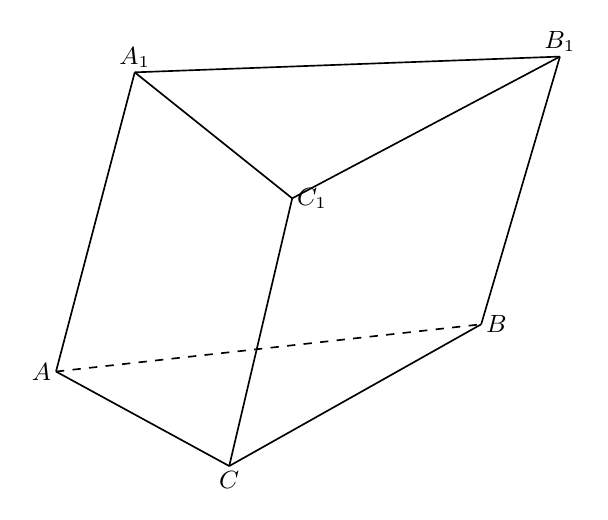
\begin{tikzpicture}[semithick, every node/.style={inner sep=1.5pt, font=\small}]
  \coordinate (A)  at (0.9,2.1);
  \coordinate (B)  at (6.3,2.7);
  \coordinate (C)  at (3.1,0.9);
  \coordinate (A1) at (1.9,5.9);
  \coordinate (B1) at (7.3,6.1);
  \coordinate (C1) at (3.9,4.3);

  % 可见棱
  \draw (A1) -- (B1);
  \draw (A1) -- (A);
  \draw (B1) -- (B);
  \draw (A1) -- (C1);
  \draw (B1) -- (C1);
  \draw (C1) -- (C);
  \draw (C) -- (A);
  \draw (C) -- (B);

  % 被遮挡的棱
  \draw[dashed] (A) -- (B);

  % 标签
  \node[above] at (A1) {$A_1$};
  \node[above] at (B1) {$B_1$};
  \node[right] at (C1) {$C_1$};
  \node[left] at (A) {$A$};
  \node[right] at (B) {$B$};
  \node[below] at (C) {$C$};
\end{tikzpicture}
\end{center}
\nopagebreak[4]
\Needspace{4\baselineskip}
\textbf{解析}

三棱柱的高是两底面所在平行平面之间的距离，也就是侧棱 $CC_1$ 在底面法线方向上的投影长。

\Needspace{5\baselineskip}
设侧棱 $CC_1$ 与底面法线所成角为 $\gamma$。因 $CA\perp CB$，可把 $CA$，$CB$ 的方向取为底面上两条互相垂直的坐标轴方向，而 $CC_1$ 与它们的夹角分别为 $60^\circ$ 与 $45^\circ$。由方向余弦关系

\nopagebreak[4]
\[\cos^260^\circ+\cos^245^\circ+\cos^2\gamma=1,\]

即 $\dfrac14+\dfrac12+\cos^2\gamma=1$，得 $\cos^2\gamma=\dfrac14$。高为正，故 $\cos\gamma=\dfrac12$。

\Needspace{5\baselineskip}
于是高

\nopagebreak[4]
\[h=CC_1\cdot\cos\gamma=1\times\frac12=\frac12.\]

选（A）。

（也可用向量验证：取 $C$ 为原点，$CA$ 为 $x$ 轴、$CB$ 为 $y$ 轴，设 $CC_1$ 方向的单位向量为 $\boldsymbol u=(u_1,u_2,u_3)$，则 $u_1=\cos60^\circ=\dfrac12$，$u_2=\cos45^\circ=\dfrac{\sqrt2}{2}$，由 $u_1^2+u_2^2+u_3^2=1$ 得 $u_3^2=\dfrac14$，高即 $|u_3|=\dfrac12$。）

\gkanswer{答案：A。}

\end{answer}
\begin{answer}
\gksolhead{7}{}

\textbf{题目}：

函数 $y=\cos\left(2x+\dfrac\pi6\right)-2$ 的图象 $F$ 按向量 $\boldsymbol a$ 平移到 $F'$，$F'$ 的解析式 $y=f(x)$，当 $y=f(x)$ 为奇函数时，向量 $\boldsymbol a$ 可以等于（　）

（A）$\left(\frac\pi6,-2\right)$

（B）$\left(\frac\pi6,2\right)$

（C）$\left(-\frac\pi6,-2\right)$

（D）$\left(-\frac\pi6,2\right)$

\Needspace{4\baselineskip}
\textbf{解析}

\Needspace{5\baselineskip}
按向量 $\boldsymbol a=(m,n)$ 平移，图象上点 $(x,y)$ 变为 $(x+m,y+n)$，故 $F'$ 的解析式为

\nopagebreak[4]
\[y-n=\cos\left[2(x-m)+\frac\pi6\right]-2,\]

\Needspace{5\baselineskip}
即

\nopagebreak[4]
\[y=\cos\left(2x-2m+\frac\pi6\right)+(n-2).\]

$y=f(x)$ 为奇函数，须同时满足两个条件：常数项为零，即 $n-2=0$，故 $n=2$；余弦型函数为奇函数，即 $-2m+\dfrac\pi6=\dfrac\pi2+k\pi$（$k\in\mathbf Z$），亦即 $m=-\dfrac\pi6-\dfrac{k\pi}{2}$。

取 $k=0$ 得 $m=-\dfrac\pi6$，此时 $f(x)=\cos\left(2x+\dfrac\pi2\right)=-\sin2x$，确为奇函数。

四个选项中只有 $\left(-\dfrac\pi6,2\right)$ 符合 $n=2$ 且 $m=-\dfrac\pi6$，故选（D）。

（$k$ 取其它整数时 $m$ 依次为 $\dfrac\pi3$，$-\dfrac{2\pi}3$ 等，均不在选项中；$n=-2$ 的两个选项常数项不为零，直接排除。）

\gkanswer{答案：D。}

\end{answer}
\begin{answer}
\gksolhead{8}{}

\textbf{题目}：

在“家电下乡”活动中，某厂要将 $100$ 台洗衣机运往邻近的乡镇，现有 $4$ 辆甲型货车和 $8$ 辆乙型货车可供使用，每辆甲型货车运输费用 $400$ 元，可装洗衣机 $20$ 台；每辆乙型货车运输费用 $300$ 元，可装洗衣机 $10$ 台，若每辆至多只运一次，则该厂所花的最少运输费用为（　）

（A）$2000$ 元

（B）$2200$ 元

（C）$2400$ 元

（D）$2800$ 元

\Needspace{4\baselineskip}
\textbf{解析}

先比较单位运价：甲型车 $400\div20=20$ 元/台，乙型车 $300\div10=30$ 元/台，故在车辆数允许时应尽量用甲型车。

4 辆甲型车全部使用，运 $80$ 台，费用 $4\times400=1600$ 元；余 $100-80=20$ 台用乙型车，需 $2$ 辆，费用 $2\times300=600$ 元。合计 $2200$ 元。

核对不得更省：若只用 $3$ 辆甲型车，则余 $40$ 台需 $4$ 辆乙型车，费用 $3\times400+4\times300=1200+1200=2400$ 元；若用 $2$ 辆甲型车，余 $60$ 台需 $6$ 辆乙型车，费用 $800+1800=2600$ 元；乙型车至多 $8$ 辆，运不完 $100$ 台而不动用甲型车。故最少费用为 $2200$ 元，选（B）。

\gkanswer{答案：B。}

\end{answer}
\begin{answer}
\gksolhead{9}{}

\textbf{题目}：

设 $x\in\mathbf R$，记不超过 $x$ 的最大整数为 $[x]$，令 $\{x\}=x-[x]$，则 $\left\{\dfrac{\sqrt5+1}{2}\right\}$，$\left[\dfrac{\sqrt5+1}{2}\right]$，$\dfrac{\sqrt5+1}{2}$（　）

（A）是等差数列但不是等比数列

（B）是等比数列但不是等差数列

（C）既是等差数列又是等比数列

（D）既不是等差数列也不是等比数列

\Needspace{4\baselineskip}
\textbf{解析}

\Needspace{5\baselineskip}
记 $\varphi=\dfrac{\sqrt5+1}{2}$。由 $\varphi^2=\varphi+1$ 得

\nopagebreak[4]
\[\varphi(\varphi-1)=\varphi^2-\varphi=1,\]

且 $1<\varphi<2$，故 $[\varphi]=1$，$\{\varphi\}=\varphi-[\varphi]=\varphi-1$。

\Needspace{5\baselineskip}
三个数依次为

\nopagebreak[4]
\[\varphi-1=\frac{\sqrt5-1}{2},\qquad 1,\qquad \varphi=\frac{\sqrt5+1}{2}.\]

\Needspace{5\baselineskip}
等比性：中间项的平方 $1^2=1$，两端之积

\nopagebreak[4]
\[(\varphi-1)\cdot\varphi=1,\]

故 $1^2=(\varphi-1)\varphi$，三数成等比数列，公比为 $\dfrac{1}{\varphi-1}=\varphi$。

等差性：两端之和 $(\varphi-1)+\varphi=2\varphi-1=\sqrt5\approx2.236$，而中间项的 $2$ 倍为 $2$，二者不等，故不成等差数列。

所以是等比数列但不是等差数列，选（B）。

\gkanswer{答案：B。}

\end{answer}
\begin{answer}
\gksolhead{10}{}

\textbf{题目}：

古希腊人常用小石子在沙滩上摆成各种性状来研究数，例如：
\nopagebreak[4]
\begin{center}% 2009 年湖北卷文科第 10 题：三角形数与正方形数的点阵图（图 1、图 2）。
% 来源 PDF：普通高考/2009/2009湖北文.pdf，SHA-256 f60ba7a5a2fef3449fba9474fa973c616aa52a15926b3a97f0dda6b909f4c861。
% 原页：第 1 页第 2 栏中部，书页码 525。
% 重绘依据：按原页逐点重绘，点数与排列照原页。
%   图 1：三角形数 1、3、6、10，自下而上每行比下一行少一点且逐行居中（1+2+3+4 点）。
%   图 2：正方形数 1、4、9、16，为 1×1、2×2、3×3、4×4 的方阵，各组底边对齐。
%   两组末均以省略号表示后续。
\begin{tikzpicture}[x=0.46cm, y=0.46cm, semithick,
  every node/.style={inner sep=1pt, font=\small}]

  % ---------- 图 1：三角形数 ----------
  % 1
  \fill (0,0) circle (2.1pt);
  % 3
  \fill (2.4,0) circle (2.1pt);
  \fill (3.4,0) circle (2.1pt);
  \fill (2.9,1) circle (2.1pt);
  % 6
  \fill (5.8,0) circle (2.1pt);
  \fill (6.8,0) circle (2.1pt);
  \fill (7.8,0) circle (2.1pt);
  \fill (6.3,1) circle (2.1pt);
  \fill (7.3,1) circle (2.1pt);
  \fill (6.8,2) circle (2.1pt);
  % 10
  \fill (10.2,0) circle (2.1pt);
  \fill (11.2,0) circle (2.1pt);
  \fill (12.2,0) circle (2.1pt);
  \fill (13.2,0) circle (2.1pt);
  \fill (10.7,1) circle (2.1pt);
  \fill (11.7,1) circle (2.1pt);
  \fill (12.7,1) circle (2.1pt);
  \fill (11.2,2) circle (2.1pt);
  \fill (12.2,2) circle (2.1pt);
  \fill (11.7,3) circle (2.1pt);

  \node at (14.7,1.4) {$\cdots$};
  \node[below] at (0,-0.6) {$1$};
  \node[below] at (2.9,-0.6) {$3$};
  \node[below] at (6.8,-0.6) {$6$};
  \node[below] at (11.7,-0.6) {$10$};
  \node at (7.3,-2.55) {图 1};

  % ---------- 图 2：正方形数 ----------
  \begin{scope}[yshift=-3.5cm]
    % 1
    \fill (0,0) circle (2.1pt);
    % 4
    \fill (2.4,0) circle (2.1pt);
    \fill (3.4,0) circle (2.1pt);
    \fill (2.4,1) circle (2.1pt);
    \fill (3.4,1) circle (2.1pt);
    % 9
    \foreach \i in {5.8,6.8,7.8} {
      \foreach \j in {0,1,2} {
        \fill (\i,\j) circle (2.1pt);
      }
    }
    % 16
    \foreach \i in {10.2,11.2,12.2,13.2} {
      \foreach \j in {0,1,2,3} {
        \fill (\i,\j) circle (2.1pt);
      }
    }

    \node at (14.7,1.4) {$\cdots$};
    \node[below] at (0,-0.6) {$1$};
    \node[below] at (2.9,-0.6) {$4$};
    \node[below] at (6.8,-0.6) {$9$};
    \node[below] at (11.7,-0.6) {$16$};
    \node at (7.3,-2.55) {图 2};
  \end{scope}
\end{tikzpicture}
\end{center}
\nopagebreak[4]
他们研究过图 1 中的 $1$，$3$，$6$，$10$，$\cdots$，由于这些数能够表示成三角形，将其称为三角形数；类似地，称图 2 中的 $1$，$4$，$9$，$16\cdots$ 这样的数成为正方形数．下列数中及时三角形数又是正方形数的是（　）

（A）$289$

（B）$1024$

（C）$1225$

（D）$1378$

\Needspace{4\baselineskip}
\textbf{解析}

记三角形数为 $T_n=\dfrac{n(n+1)}2$，正方形数为 $m^2$。逐项检验：

\begin{itemize}
\item $289=17^2$。令 $\dfrac{n(n+1)}2=289$，即 $n^2+n-578=0$，判别式 $1+4\times578=2313$，$\sqrt{2313}\approx48.09$ 非整数，故 $289$ 不是三角形数。
\item $1024=32^2$。令 $n^2+n-2048=0$，判别式 $1+8192=8193$，$\sqrt{8193}\approx90.51$ 非整数，故 $1024$ 不是三角形数。
\item $1225=35^2$。令 $n^2+n-2450=0$，判别式 $1+9800=9801=99^2$，$n=\dfrac{-1+99}{2}=49$，而 $T_{49}=\dfrac{49\times50}{2}=1225$，故 $1225$ 既是正方形数又是三角形数。
\item $1378$。令 $n^2+n-2756=0$，判别式 $1+11024=11025=105^2$，$n=\dfrac{-1+105}{2}=52$，$T_{52}=1378$，是三角形数；但 $37^2=1369<1378<1444=38^2$，不是正方形数。
\end{itemize}

故只有 $1225$ 同时满足，选（C）。

原页本题有三处排印问题：「摆成各种性状」应为「摆成各种形状」，「这样的数成为正方形数」应为「称为正方形数」，「下列数中及时三角形数又是正方形数」应为「既是……又是……」。三者均不影响题意与答案，本库照录原页字面并登记问题。

\gkanswer{答案：C。}

\end{answer}
\begin{answer}
\gksolhead{11}{}

\textbf{题目}：

已知 $(1+ax)^5=1+10x+bx^2+\cdots+a^5x^5$，则 $b=$\gkblank{}．

\Needspace{4\baselineskip}
\textbf{解析}

\Needspace{5\baselineskip}
由二项式定理，

\nopagebreak[4]
\[(1+ax)^5=1+\mathrm C_5^1ax+\mathrm C_5^2a^2x^2+\cdots=1+5ax+10a^2x^2+\cdots+a^5x^5.\]

与所给式比较 $x$ 的系数：$5a=10$，故 $a=2$。

\Needspace{5\baselineskip}
再比较 $x^2$ 的系数：

\nopagebreak[4]
\[b=10a^2=10\times4=40.\]

也可直接由 $b=\mathrm C_5^2a^2$ 与 $a=2$ 得到同一结果。

\gkanswer{答案：$40$。}

\end{answer}
\begin{answer}
\gksolhead{12}{}

\textbf{题目}：

甲、乙、丙三人将参加某项测试，他们能达标的概率分别是 $0.8$、$0.6$、$0.5$，则三人都达标的概率是\gkblank{}，三人中至少有一人达标的概率是\gkblank{}．

\Needspace{4\baselineskip}
\textbf{解析}

三人能否达标相互独立。

\Needspace{5\baselineskip}
三人都达标：

\nopagebreak[4]
\[P_1=0.8\times0.6\times0.5=0.24.\]

\Needspace{5\baselineskip}
“至少一人达标”的对立事件是“三人都不达标”，其概率为

\nopagebreak[4]
\[(1-0.8)(1-0.6)(1-0.5)=0.2\times0.4\times0.5=0.04.\]

\Needspace{5\baselineskip}
故至少一人达标的概率

\nopagebreak[4]
\[P_2=1-0.04=0.96.\]

核对：$P_2\geqslant P_1$，且 $P_1+P(\text{\text{恰有两人}})+P(\text{\text{恰有一人}})=0.96$ 与逐项计算一致。

\gkanswer{答案：$0.24$；$0.96$。}

\end{answer}
\begin{answer}
\gksolhead{13}{}

\textbf{题目}：

设集合 $A=\{x\mid\log_2x<1\}$，$B=\left\{x\mid\dfrac{x-1}{x+2}<1\right\}$，则 $A\cap B=$\gkblank{}．

\Needspace{4\baselineskip}
\textbf{解析}

\Needspace{5\baselineskip}
先化简 $A$。$\log_2x<1$ 要求真数为正，即 $x>0$；在此前提下 $\log_2x<1=\log_22$，得 $x<2$。故

\nopagebreak[4]
\[A=\{x\mid0<x<2\}=(0,2).\]

\Needspace{5\baselineskip}
再化简 $B$。注意 $x\neq-2$。

\nopagebreak[4]
\[\frac{x-1}{x+2}<1\iff\frac{x-1}{x+2}-1<0\iff\frac{(x-1)-(x+2)}{x+2}<0\iff\frac{-3}{x+2}<0.\]

\Needspace{5\baselineskip}
分子为负常数，故只需分母为正：$x+2>0$，即 $x>-2$。故

\nopagebreak[4]
\[B=(-2,+\infty).\]

\Needspace{5\baselineskip}
取交集：

\nopagebreak[4]
\[A\cap B=(0,2)\cap(-2,+\infty)=(0,2).\]

端点检验：$x=0$ 不满足 $\log_2x<1$（无定义），不可取；$x=2$ 使 $\log_2x=1$，不满足严格小于，不可取；$x=-2$ 使 $B$ 的分母为零，不可取。故为开区间 $(0,2)$。

\gkanswer{答案：$(0,2)$。}

\end{answer}
\begin{answer}
\gksolhead{14}{}

\textbf{题目}：

过原点 $O$ 作圆 $x^2+y^2-6x-8y+20=0$ 的两条切线，设切点分别为 $P$、$Q$，则线段 $PQ$ 的长为\gkblank{}．

\Needspace{4\baselineskip}
\textbf{解析}

\Needspace{5\baselineskip}
配方：

\nopagebreak[4]
\[x^2+y^2-6x-8y+20=0\iff(x-3)^2+(y-4)^2=5,\]

圆心 $C(3,4)$，半径 $r=\sqrt5$，$|OC|=\sqrt{3^2+4^2}=5>r$，故过原点可作两条切线。

\Needspace{5\baselineskip}
两切点 $P$，$Q$ 的连线（切点弦）是点 $O$ 关于该圆的极线。对圆 $x^2+y^2-6x-8y+20=0$，点 $(x_0,y_0)$ 的极线为

\nopagebreak[4]
\[x_0x+y_0y-3(x+x_0)-4(y+y_0)+20=0,\]

\Needspace{5\baselineskip}
代入 $(x_0,y_0)=(0,0)$ 得

\nopagebreak[4]
\[-3x-4y+20=0,\qquad\text{\text{即}}\quad3x+4y=20.\]

\Needspace{5\baselineskip}
圆心 $C(3,4)$ 到该直线的距离

\nopagebreak[4]
\[d=\frac{|3\times3+4\times4-20|}{\sqrt{3^2+4^2}}=\frac{5}{5}=1.\]

\Needspace{5\baselineskip}
弦长的一半为 $\sqrt{r^2-d^2}=\sqrt{5-1}=2$，故

\nopagebreak[4]
\[|PQ|=2\times2=4.\]

数值校验：切线长 $|OP|=\sqrt{|OC|^2-r^2}=\sqrt{25-5}=2\sqrt5$；在直角三角形 $OPC$ 中，斜边上的高 $h=\dfrac{|OP|\cdot r}{|OC|}=\dfrac{2\sqrt5\cdot\sqrt5}{5}=2$，恰为 $\dfrac{|PQ|}{2}$，与上面所得一致。

\gkanswer{答案：$4$。}

\end{answer}
\begin{answer}
\gksolhead{15}{}

\textbf{题目}：

下图是样本容量为 $200$ 的频率分布直方图．
\nopagebreak[4]
\begin{center}% 2009 年湖北卷文科第 15 题：样本容量 200 的频率分布直方图。
% 来源 PDF：普通高考/2009/2009湖北文.pdf，SHA-256 f60ba7a5a2fef3449fba9474fa973c616aa52a15926b3a97f0dda6b909f4c861。
% 原页：第 1 页第 2 栏下部，书页码 525。
% 重绘依据：横轴 0—22，0 与 2 之间为省略断轴；纵轴为「频率/组距」，组距 4。
%   五组矩形高：[2,6)=0.02，[6,10)=0.08，[10,14)=0.09，[14,18)=0.03，[18,22)=0.03；
%   0.02+0.08+0.09+0.03+0.03=0.25，乘组距 4 恰为 1，已核对。
%   虚线标出 0.02、0.03、0.08、0.09 四条水平参考线，位置照原页。
%   纵轴标题置于轴顶右侧、0.09 虚线之上，避开 0.09/0.08 刻度字与虚线。
\begin{tikzpicture}[x=0.34cm, y=30cm, semithick,
  every node/.style={inner sep=1.2pt, font=\small}]

  % 水平虚线参考线（画在矩形之下，白色填充的矩形覆盖其内部）
  \draw[dashed] (0,0.09) -- (10,0.09);
  \draw[dashed] (0,0.08) -- (10,0.08);
  \draw[dashed] (10,0.03) -- (22,0.03);
  \draw[dashed] (0,0.02) -- (2,0.02);

  % 各组矩形
  \draw[fill=white] (2,0) rectangle (6,0.02);
  \draw[fill=white] (6,0) rectangle (10,0.08);
  \draw[fill=white] (10,0) rectangle (14,0.09);
  \draw[fill=white] (14,0) rectangle (18,0.03);
  \draw[fill=white] (18,0) rectangle (22,0.03);

  % 坐标轴
  \draw[-{Stealth}] (-0.5,0) -- (23.4,0) node[right, inner sep=3pt] {样本数据};
  \draw[-{Stealth}] (0,-0.002) -- (0,0.1125);
  \node[anchor=west] at (0.45,0.1045) {频率/组距};

  % 断轴符号（0 与 2 之间）
  \draw (0.45,0) -- (0.58,0.0022) -- (0.71,0) -- (0.84,0.0022) -- (0.97,0);

  % 刻度与标签
  \foreach \x in {2,6,10,14,18,22} {
    \draw (\x,0) -- (\x,-0.0012);
    \node[below] at (\x,-0.0018) {$\x$};
  }
  \node[below left=1pt] at (0,0) {$O$};

  % 纵轴刻度标签
  \foreach \h/\t in {0.02/0.02, 0.03/0.03, 0.08/0.08, 0.09/0.09} {
    \node[left, font=\scriptsize] at (0,\h) {\t};
  }
\end{tikzpicture}
\end{center}
\nopagebreak[4]
根据样本的频率分布直方图估计，样本数据落在 $[6,10)$ 内的频数为\gkblank{}，数据落在 $[2,10)$ 内的概率约为\gkblank{}．

\Needspace{4\baselineskip}
\textbf{解析}

\Needspace{5\baselineskip}
组距为 $22-18=4$。设五组 $[2,6)$，$[6,10)$，$[10,14)$，$[14,18)$，$[18,22)$ 的高依次为 $h_1,\dots,h_5$。由直方图读出

\nopagebreak[4]
\[h_1=0.02,\quad h_2=0.08,\quad h_3=0.09,\quad h_4=0.03,\quad h_5=0.03.\]

\Needspace{5\baselineskip}
核对总面积：

\nopagebreak[4]
\[(h_1+h_2+h_3+h_4+h_5)\times4=(0.02+0.08+0.09+0.03+0.03)\times4=0.25\times4=1,\]

与“各矩形面积之和为 $1$”一致，说明读数无误。

\Needspace{5\baselineskip}
$[6,10)$ 内的频率为 $h_2\times4=0.08\times4=0.32$，样本容量 $200$，故频数

\nopagebreak[4]
\[0.32\times200=64.\]

$[2,10)$ 内的频率为 $(h_1+h_2)\times4=(0.02+0.08)\times4=0.4$，用频率估计概率得 $0.4$。

\gkanswer{答案：$64$；$0.4$。}

\end{answer}
\begin{answer}
\gksolhead{16}{}

\textbf{题目}：

在锐角 $\triangle ABC$ 中，$a$、$b$、$c$ 分别为角 $A$、$B$、$C$ 所对的边，且 $\sqrt3a=2c\sin A$．

（1）确定角 $C$ 的大小；

（2）若 $c=\sqrt7$，且 $\triangle ABC$ 的面积为 $\dfrac{3\sqrt3}{2}$，求 $a+b$ 的值．

\Needspace{4\baselineskip}
\textbf{解析}

\Needspace{5\baselineskip}
（1）由正弦定理 $\dfrac{a}{\sin A}=\dfrac{c}{\sin C}$ 得 $\sin A=\dfrac{a\sin C}{c}$。代入已知条件：

\nopagebreak[4]
\[\sqrt3a=2c\sin A=2c\cdot\frac{a\sin C}{c}=2a\sin C.\]

因 $a>0$，两边除以 $a$ 得 $\sin C=\dfrac{\sqrt3}{2}$。

又 $\triangle ABC$ 为锐角三角形，三个内角均为锐角，故 $0<C<\dfrac\pi2$，只能取 $C=\dfrac\pi3$。

\Needspace{5\baselineskip}
（2）由面积公式

\nopagebreak[4]
\[S=\frac12ab\sin C=\frac12ab\cdot\frac{\sqrt3}{2}=\frac{\sqrt3}{4}ab=\frac{3\sqrt3}{2},\]

得 $ab=6$。

\Needspace{5\baselineskip}
由余弦定理，$c=\sqrt7$，$C=\dfrac\pi3$：

\nopagebreak[4]
\[c^2=a^2+b^2-2ab\cos C=a^2+b^2-ab.\]

\Needspace{5\baselineskip}
代入 $c^2=7$，$ab=6$ 得 $a^2+b^2=7+6=13$。于是

\nopagebreak[4]
\[(a+b)^2=a^2+b^2+2ab=13+12=25,\]

因 $a$，$b$ 为正，故 $a+b=5$。

校验：$a+b=5$，$ab=6$ 给出 $\{a,b\}=\{2,3\}$，此时 $c^2=4+9-6=7$，$S=\dfrac{\sqrt3}{4}\times6=\dfrac{3\sqrt3}{2}$，且三边 $2,3,\sqrt7$ 中 $\sqrt7\approx2.65$ 所对角的余弦为 $\dfrac{4+9-7}{12}=\dfrac12$，三角形确为锐角三角形，符合题意。

\gkanswer{答案：（1）$\dfrac\pi3$；（2）$5$。}

\end{answer}
\begin{answer}
\gksolhead{17}{}

\textbf{题目}：

围建一个面积为 $360\ \mathrm{m^2}$ 的矩形场地，要求矩形场地的一面利用旧墙（利用旧墙需维修），其它三面围墙要新建，在旧墙的对面的新墙上要留一个宽度为 $2\ \mathrm m$ 的进出口．如图所示，已知旧墙的维修费用为 $45$ 元/m，新墙的造价为 $180$ 元/m．设利用的旧墙的长度为 $x$（单位：m），修建此矩形场地围墙的总费用为 $y$（单位：元）．

（1）将 $y$ 表示为 $x$ 的函数；

（2）试确定 $x$，使修建此矩形场地围墙的总费用最小，并求出最小总费用．
\nopagebreak[4]
\begin{center}% 2009 年湖北卷文科第 17 题：矩形场地与旧墙。
% 来源 PDF：普通高考/2009/2009湖北文.pdf，SHA-256 f60ba7a5a2fef3449fba9474fa973c616aa52a15926b3a97f0dda6b909f4c861。
% 原页：第 1 页第 3 栏中部，书页码 525。
% 重绘依据：照原页方位，旧墙在上方并画成带竖缝的墙身，左右两侧为新墙，
%   与旧墙相对的新墙在中间留出宽度 2 m 的进出口（缺口）；x 为所利用旧墙的长度，
%   用双箭头标在矩形内侧上方。图不按比例，只表示位置关系。
\begin{tikzpicture}[x=1cm, y=1cm, semithick,
  every node/.style={inner sep=1.5pt, font=\small}]

  % 旧墙墙身
  \draw[thick] (-0.75,0.40) -- (6.75,0.40);
  \draw[thick] (-0.75,0.06) -- (6.75,0.06);
  \foreach \xx in {-0.45,-0.15,0.15,...,6.75} {
    \draw (\xx,0.06) -- (\xx,0.40);
    \draw (\xx,0.40) -- (\xx,0.52);
    \draw (\xx,0.06) -- (\xx,-0.06);
  }

  % 左右两侧新墙
  \draw (0,0.06) -- (0,-2.75);
  \draw (6,0.06) -- (6,-2.75);

  % 与旧墙相对的新墙，中部留 2 m 进出口
  \draw (0,-2.75) -- (2.65,-2.75);
  \draw (3.35,-2.75) -- (6,-2.75);

  % 旧墙长度 x
  \draw[{Stealth}-{Stealth}] (0,-0.85) -- (6,-0.85)
    node[midway, above] {$x$};
\end{tikzpicture}
\end{center}
\nopagebreak[4]
\Needspace{4\baselineskip}
\textbf{解析}

（1）设利用的旧墙长为 $x$，则矩形另一边长为 $\dfrac{360}{x}$。与旧墙相对的墙长为 $x$，其上留 $2\ \mathrm m$ 的进出口，实际新建长度为 $x-2$；另两面新墙各长 $\dfrac{360}{x}$。因为要留出进出口，须 $x>2$。

\Needspace{5\baselineskip}
费用：旧墙维修 $45x$ 元；新墙总长 $x-2+\dfrac{720}{x}$，造价 $180\left(x-2+\dfrac{720}{x}\right)$ 元。故

\nopagebreak[4]
\[y=45x+180\left(x-2+\frac{720}{x}\right)=45x+180x-360+\frac{129600}{x},\]

\Needspace{5\baselineskip}
即

\nopagebreak[4]
\[y=225x+\frac{129600}{x}-360\quad(x>2).\]

\Needspace{5\baselineskip}
（2）因 $x>0$，由均值不等式

\nopagebreak[4]
\[225x+\frac{129600}{x}\geqslant2\sqrt{225x\cdot\frac{129600}{x}}=2\sqrt{29160000}=2\times5400=10800,\]

\Needspace{5\baselineskip}
等号当且仅当

\nopagebreak[4]
\[225x=\frac{129600}{x}\iff x^2=\frac{129600}{225}=576\iff x=24,\]

且 $24>2$ 满足定义域。此时另一边长为 $\dfrac{360}{24}=15$。

\Needspace{5\baselineskip}
最小总费用

\nopagebreak[4]
\[y_{\min}=10800-360=10440\ (\text{\text{元}}).\]

校验：$x=24$ 时直接代入原式 $45\times24+180\left(22+2\times15\right)=1080+180\times52=1080+9360=10440$，与上式一致。再取 $x=23$：$y=225\times23+\dfrac{129600}{23}-360=5175+5634.8-360\approx10449.8>10440$；取 $x=25$：$y=5625+5184-360=10449>10440$，确为最小。

\gkanswer{答案：（1）$y=225x+\dfrac{129600}{x}-360$（$x>2$）；（2）$x=24$，最小总费用 $10440$ 元。}

\end{answer}
\begin{answer}
\gksolhead{18}{}

\textbf{题目}：

如图，四棱锥 $S-ABCD$ 的底面是正方形，$SD\perp$ 平面 $ABCD$，$SD=AD=a$，点 $E$ 是 $SD$ 上的点，且 $DE=\lambda a$（$0<\lambda\leqslant1$）．

（1）求证：对任意的 $\lambda\in(0,1]$，都有 $AC\perp BE$；

（2）若二面角 $C-AE-D$ 的大小为 $60^\circ$，求 $\lambda$ 的值．
\nopagebreak[4]
\begin{center}% 2009 年湖北卷文科第 18 题：四棱锥 S-ABCD。
% 来源 PDF：普通高考/2009/2009湖北文.pdf，SHA-256 f60ba7a5a2fef3449fba9474fa973c616aa52a15926b3a97f0dda6b909f4c861。
% 原页：第 2 页第 1 栏上部，书页码 526。
% 重绘依据：底面 ABCD 为正方形，SD⊥底面，故 SD 画成竖直线并落到底面顶点 D 上；
%   D 在锥体内部，SD、DA、DC、AC 与 E 到 A、C 的连线均被遮挡，画虚线；
%   SA、SB、SC、AB、BC 为可见棱，画实线。E 为 SD 上一点（DE=λa）。
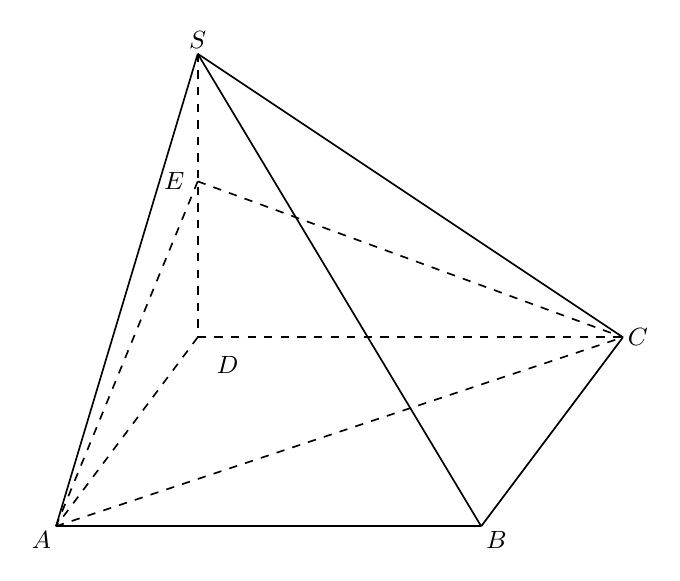
\begin{tikzpicture}[semithick, every node/.style={inner sep=1.5pt, font=\small}]
  \coordinate (A) at (0.2,1.2);
  \coordinate (B) at (5.6,1.2);
  \coordinate (C) at (7.4,3.6);
  \coordinate (D) at (2.0,3.6);
  \coordinate (S) at (2.0,7.2);
  \coordinate (E) at (2.0,5.58);

  % 可见棱
  \draw (S) -- (A);
  \draw (S) -- (B);
  \draw (S) -- (C);
  \draw (A) -- (B);
  \draw (B) -- (C);

  % 被遮挡的棱
  \draw[dashed] (S) -- (D);
  \draw[dashed] (D) -- (A);
  \draw[dashed] (D) -- (C);
  \draw[dashed] (A) -- (C);
  \draw[dashed] (E) -- (A);
  \draw[dashed] (E) -- (C);

  % 标签
  \node[above] at (S) {$S$};
  \node[left=3pt] at (E) {$E$};
  \node[below right=5pt] at (D) {$D$};
  \node[below left] at (A) {$A$};
  \node[below right] at (B) {$B$};
  \node[right] at (C) {$C$};
\end{tikzpicture}
\end{center}
\nopagebreak[4]
\Needspace{4\baselineskip}
\textbf{解析}

\Needspace{5\baselineskip}
（1）以 $D$ 为原点，$\overrightarrow{DA}$，$\overrightarrow{DC}$，$\overrightarrow{DS}$ 的方向分别为 $x$，$y$，$z$ 轴正方向建立空间直角坐标系。由 $SD=AD=a$ 且底面为正方形得

\nopagebreak[4]
\[D(0,0,0),\quad A(a,0,0),\quad C(0,a,0),\quad B(a,a,0),\quad S(0,0,a).\]

\Needspace{5\baselineskip}
点 $E$ 在 $SD$ 上且 $DE=\lambda a$，故 $E(0,0,\lambda a)$。于是

\nopagebreak[4]
\[\overrightarrow{AC}=(0,a,0)-(a,0,0)=(-a,a,0),\qquad
\overrightarrow{BE}=(0,0,\lambda a)-(a,a,0)=(-a,-a,\lambda a).\]

\nopagebreak[4]
\[\overrightarrow{AC}\cdot\overrightarrow{BE}=(-a)(-a)+a\cdot(-a)+0\cdot\lambda a=a^2-a^2=0.\]

故 $AC\perp BE$，对任意 $\lambda\in(0,1]$ 都成立。

（2）平面 $AED$ 由 $A(a,0,0)$，$E(0,0,\lambda a)$，$D(0,0,0)$ 确定，三点 $y$ 坐标均为 $0$，故该平面即 $y=0$，法向量可取 $\boldsymbol n_1=(0,1,0)$。

\Needspace{5\baselineskip}
平面 $CAE$ 中

\nopagebreak[4]
\[\overrightarrow{CA}=(a,-a,0),\qquad \overrightarrow{CE}=(0,-a,\lambda a).\]

\Needspace{5\baselineskip}
法向量

\nopagebreak[4]
\[\boldsymbol n_2=\overrightarrow{CA}\times\overrightarrow{CE}
=\begin{vmatrix}\boldsymbol i&\boldsymbol j&\boldsymbol k\\ a&-a&0\\ 0&-a&\lambda a\end{vmatrix}
=(-\lambda a^2,\ -\lambda a^2,\ -a^2),\]

可取 $\boldsymbol n_2=(\lambda,\lambda,1)$。

\Needspace{5\baselineskip}
二面角 $C-AE-D$ 的大小为 $60^\circ$，故

\nopagebreak[4]
\[\cos60^\circ=\frac{|\boldsymbol n_1\cdot\boldsymbol n_2|}{|\boldsymbol n_1||\boldsymbol n_2|}
=\frac{\lambda}{1\cdot\sqrt{2\lambda^2+1}}.\]

\Needspace{5\baselineskip}
即 $\dfrac12=\dfrac{\lambda}{\sqrt{2\lambda^2+1}}$，亦即 $\sqrt{2\lambda^2+1}=2\lambda$。两边平方：

\nopagebreak[4]
\[2\lambda^2+1=4\lambda^2\quad\Longrightarrow\quad2\lambda^2=1\quad\Longrightarrow\quad\lambda^2=\frac12.\]

因 $\lambda>0$，得 $\lambda=\dfrac{\sqrt2}{2}$，且 $\dfrac{\sqrt2}{2}\in(0,1]$，符合题意。

（几何校验：$\lambda=\dfrac{\sqrt2}{2}$ 时 $\cos60^\circ=\dfrac{\sqrt2/2}{\sqrt{1+1}}=\dfrac12$，与题设一致；$\lambda=\dfrac12$ 时 $\cos\theta=\dfrac{1/2}{\sqrt{3/2}}=\dfrac{\sqrt6}{6}\approx0.408$，二面角约 $65.9^\circ$，不等于 $60^\circ$，说明解唯一。）

\gkanswer{答案：（1）证明见解析；（2）$\dfrac{\sqrt2}{2}$。}

\end{answer}
\begin{answer}
\gksolhead{19}{}

\textbf{题目}：

已知 $\{a_n\}$ 是一个公差大于 $0$ 的等差数列，且满足 $a_3a_6=55$，$a_2+a_7=16$．

（1）求数列 $\{a_n\}$ 的通项公式；

（2）若数列 $\{a_n\}$ 和数列 $\{b_n\}$ 满足等式：$a_n=\dfrac{b_1}{2}+\dfrac{b_2}{2^2}+\dfrac{b_3}{2^3}+\cdots+\dfrac{b_n}{2^n}$（$n$ 为正整数），求数列 $\{b_n\}$ 的前 $n$ 项和 $S_n$．

\Needspace{4\baselineskip}
\textbf{解析}

\Needspace{5\baselineskip}
（1）设公差为 $d>0$，首项为 $a_1$。由等差数列性质

\nopagebreak[4]
\[a_2+a_7=a_3+a_6=16.\]

\Needspace{5\baselineskip}
又 $a_3a_6=55$，故 $a_3$，$a_6$ 是方程

\nopagebreak[4]
\[t^2-16t+55=0\]

的两根，解得 $t=5$ 或 $t=11$。因 $d>0$，$a_6>a_3$，故 $a_3=5$，$a_6=11$。

\Needspace{5\baselineskip}
于是 $3d=a_6-a_3=6$，$d=2$，$a_1=a_3-2d=5-4=1$。通项

\nopagebreak[4]
\[a_n=1+2(n-1)=2n-1.\]

校验：$a_3=5$，$a_6=11$，$a_3a_6=55$；$a_2+a_7=3+13=16$，符合。

\Needspace{5\baselineskip}
（2）由

\nopagebreak[4]
\[a_n=\frac{b_1}{2}+\frac{b_2}{2^2}+\cdots+\frac{b_n}{2^n}\]

得 $n=1$ 时 $a_1=\dfrac{b_1}{2}$，而 $a_1=1$，故 $b_1=2$。

\Needspace{5\baselineskip}
当 $n\geqslant2$ 时，将 $n$ 与 $n-1$ 两式相减：

\nopagebreak[4]
\[\frac{b_n}{2^n}=a_n-a_{n-1}=(2n-1)-(2n-3)=2,\]

故 $b_n=2\cdot2^n=2^{n+1}$（$n\geqslant2$）。

\Needspace{5\baselineskip}
于是前 $n$ 项和

\nopagebreak[4]
\[S_n=b_1+b_2+\cdots+b_n=2+\left(2^3+2^4+\cdots+2^{n+1}\right).\]

\Needspace{5\baselineskip}
括号内是首项 $8$、公比 $2$、共 $n-1$ 项的等比数列之和：

\nopagebreak[4]
\[2^3+2^4+\cdots+2^{n+1}=8\cdot\frac{2^{n-1}-1}{2-1}=2^{n+2}-8.\]

\Needspace{5\baselineskip}
故

\nopagebreak[4]
\[S_n=2+2^{n+2}-8=2^{n+2}-6.\]

校验：$n=1$ 时 $S_1=2^3-6=2=b_1$；$n=2$ 时 $S_2=2^4-6=10=b_1+b_2=2+8$；$n=3$ 时 $S_3=2^5-6=26=2+8+16$，均一致。

\gkanswer{答案：（1）$a_n=2n-1$；（2）$S_n=2^{n+2}-6$。}

\end{answer}
\begin{answer}
\gksolhead{20}{}

\textbf{题目}：

如图，过抛物线 $y^2=2px$（$p>0$）的焦点 $F$ 的直线与抛物线相交于 $M$、$N$ 两点，自 $M$、$N$ 向准线 $l$ 作垂线，垂足分别为 $M_1$、$N_1$．

（1）求证：$FM_1\perp FN_1$；

（2）记 $\triangle FMM_1$、$\triangle FM_1N_1$、$\triangle FNN_1$ 的面积分别为 $S_1$、$S_2$、$S_3$，试判断 $S_2^2=4S_1S_3$ 是否成立，并证明你的结论．
\nopagebreak[4]
\begin{center}% 2009 年湖北卷文科第 20 题：抛物线与准线。
% 来源 PDF：普通高考/2009/2009湖北文.pdf，SHA-256 f60ba7a5a2fef3449fba9474fa973c616aa52a15926b3a97f0dda6b909f4c861。
% 原页：第 2 页第 2 栏中部，书页码 526。
% 重绘依据：抛物线 y^2=2px（取 p=1 作图），焦点 F，准线 l 在 y 轴左侧；
%   过 F 的直线交抛物线于 M（上）、N（下），M1、N1 为 M、N 在 l 上的垂足；
%   M1M、N1N 水平，FM1、FN1 与 MN 均按原页画出。
%   标注位置按几何避让：M1、N1 左移让开准线与水平垂线段；O、N 置于准线与
%   y 轴之间的空档（O 在 N1N 之上，N 在 N1N 之下、直线 MN 之上）；F 下移让开直线 MN。
\begin{tikzpicture}[x=1.3cm, y=1.3cm, semithick,
  every node/.style={inner sep=1.2pt, font=\small}]

  % 坐标轴
  \draw[-{Stealth}] (-1.25,0) -- (3.95,0) node[right, inner sep=3pt] {$x$};
  \draw[-{Stealth}] (0,-2.15) -- (0,2.95) node[above, inner sep=3pt] {$y$};

  % 准线
  \draw (-0.5,-2.15) -- (-0.5,2.85);
  \node[left=2pt] at (-0.5,2.55) {$l$};

  % 抛物线 y^2=2x 的上下两支
  \draw[domain=0:3.55, samples=120, smooth]
    plot (\x,{sqrt(2*\x)});
  \draw[domain=0:3.55, samples=120, smooth]
    plot (\x,{-sqrt(2*\x)});

  % 过焦点 F 的直线（斜率 1.6），交抛物线于 M、N
  \coordinate (F)  at (0.5,0);
  \coordinate (M)  at (1.627,1.803);
  \coordinate (N)  at (0.154,-0.554);
  \coordinate (M1) at (-0.5,1.803);
  \coordinate (N1) at (-0.5,-0.554);
  \draw (-0.12,-0.99) -- (2.55,3.28);

  % 垂线段与两腰
  \draw (M1) -- (M);
  \draw (N1) -- (N);
  \draw (F) -- (M1);
  \draw (F) -- (N1);

  % 标签
  \node[left=4pt] at (M1) {$M_1$};
  \node[below right=3pt] at (M) {$M$};
  \node[left=4pt] at (N1) {$N_1$};
  \node at (-0.25,-0.78) {$N$};
  \node at (-0.25,-0.20) {$O$};
  \node at (0.62,-0.18) {$F$};
\end{tikzpicture}
\end{center}
\nopagebreak[4]
\Needspace{4\baselineskip}
\textbf{解析}

\Needspace{5\baselineskip}
（1）设 $M(x_1,y_1)$，$N(x_2,y_2)$。抛物线 $y^2=2px$ 的焦点 $F\left(\dfrac p2,0\right)$，准线 $l:x=-\dfrac p2$，故

\nopagebreak[4]
\[M_1\left(-\frac p2,y_1\right),\qquad N_1\left(-\frac p2,y_2\right).\]

\Needspace{5\baselineskip}
过 $F$ 的直线若不垂直于 $x$ 轴，可设为 $x=my+\dfrac p2$，代入 $y^2=2px$：

\nopagebreak[4]
\[y^2=2p\left(my+\frac p2\right)=2pmy+p^2,\]

\Needspace{5\baselineskip}
即 $y^2-2pmy-p^2=0$，由韦达定理

\nopagebreak[4]
\[y_1y_2=-p^2.\]

若直线垂直于 $x$ 轴，则 $x=\dfrac p2$，$y^2=p^2$，$y_{1,2}=\pm p$，仍有 $y_1y_2=-p^2$。

\Needspace{5\baselineskip}
于是

\nopagebreak[4]
\[\overrightarrow{FM_1}=\left(-\frac p2-\frac p2,\ y_1-0\right)=(-p,y_1),\qquad
\overrightarrow{FN_1}=(-p,y_2),\]

\nopagebreak[4]
\[\overrightarrow{FM_1}\cdot\overrightarrow{FN_1}=(-p)(-p)+y_1y_2=p^2-p^2=0,\]

故 $FM_1\perp FN_1$。

（2）$S_2^2=4S_1S_3$ 成立。

由抛物线定义，$M$ 到准线的距离等于到焦点的距离，即 $|MM_1|=x_1+\dfrac p2$；同理 $|NN_1|=x_2+\dfrac p2$。

\Needspace{5\baselineskip}
$\triangle FMM_1$ 以 $MM_1$ 为底时，$F$ 到直线 $MM_1$（即水平线 $y=y_1$）的距离为 $|y_1|$，故

\nopagebreak[4]
\[S_1=\frac12\left(x_1+\frac p2\right)|y_1|,\qquad
S_3=\frac12\left(x_2+\frac p2\right)|y_2|.\]

\Needspace{5\baselineskip}
$\triangle FM_1N_1$ 以 $M_1N_1$ 为底，$|M_1N_1|=|y_1-y_2|$，$F$ 到准线的距离为 $p$，故

\nopagebreak[4]
\[S_2=\frac12p|y_1-y_2|.\]

\Needspace{5\baselineskip}
由 $y_1y_2=-p^2$ 及 $y_i^2=2px_i$ 得

\nopagebreak[4]
\[x_1x_2=\frac{y_1^2}{2p}\cdot\frac{y_2^2}{2p}=\frac{(y_1y_2)^2}{4p^2}=\frac{p^2}{4},\qquad
x_1+x_2=\frac{y_1^2+y_2^2}{2p}.\]

\Needspace{5\baselineskip}
于是

\nopagebreak[4]
\[\left(x_1+\frac p2\right)\left(x_2+\frac p2\right)
=x_1x_2+\frac p2(x_1+x_2)+\frac{p^2}{4}
=\frac{p^2}{2}+\frac{y_1^2+y_2^2}{4}.\]

\Needspace{5\baselineskip}
又 $y_1^2+y_2^2=(y_1+y_2)^2-2y_1y_2=(y_1+y_2)^2+2p^2$，故

\nopagebreak[4]
\[\left(x_1+\frac p2\right)\left(x_2+\frac p2\right)
=\frac{p^2}{2}+\frac{(y_1+y_2)^2+2p^2}{4}
=\frac{(y_1+y_2)^2+4p^2}{4}.\]

\Needspace{5\baselineskip}
而 $(y_1+y_2)^2-4y_1y_2=(y_1-y_2)^2$，结合 $y_1y_2=-p^2$ 得 $(y_1+y_2)^2+4p^2=(y_1-y_2)^2$。所以

\nopagebreak[4]
\[\left(x_1+\frac p2\right)\left(x_2+\frac p2\right)=\frac{(y_1-y_2)^2}{4}.\]

\Needspace{5\baselineskip}
代入 $S_1$，$S_3$：

\nopagebreak[4]
\[S_1S_3=\frac14\cdot\frac{(y_1-y_2)^2}{4}\cdot|y_1y_2|
=\frac{p^2(y_1-y_2)^2}{16},\]

\Needspace{5\baselineskip}
而

\nopagebreak[4]
\[S_2^2=\frac{p^2(y_1-y_2)^2}{4}=4\cdot\frac{p^2(y_1-y_2)^2}{16}=4S_1S_3.\]

故 $S_2^2=4S_1S_3$ 成立。

\gkanswer{答案：（1）证明见解析；（2）$S_2^2=4S_1S_3$ 成立。}

\end{answer}
\begin{answer}
\gksolhead{21}{}

\textbf{题目}：

已知关于 $x$ 的函数 $f(x)=-\dfrac13x^3+bx^2+cx+bc$，其导函数为 $f'(x)$．令 $g(x)=|f'(x)|$，记函数 $g(x)$ 在区间 $[-1,1]$ 上的最大值为 $M$．

（1）如果函数 $f(x)$ 在 $x=1$ 处有极值 $-\dfrac43$，试确定 $b$、$c$ 的值；

（2）若 $|b|>1$，证明对任意的 $c$，都有 $M>2$；

（3）若 $M\geqslant k$ 对任意的 $b$、$c$ 恒成立，试求 $k$ 的最大值．

\Needspace{4\baselineskip}
\textbf{解析}

\Needspace{5\baselineskip}
（1）求导：

\nopagebreak[4]
\[f'(x)=-x^2+2bx+c.\]

由 $f$ 在 $x=1$ 处有极值 $-\dfrac43$，须 $f'(1)=0$ 且 $f(1)=-\dfrac43$。

$f'(1)=-1+2b+c=0$，故 $c=1-2b$。

\Needspace{5\baselineskip}
$f(1)=-\dfrac13+b+c+bc=-\dfrac43$，即

\nopagebreak[4]
\[b+c+bc=-1.\]

\Needspace{5\baselineskip}
代入 $c=1-2b$：

\nopagebreak[4]
\[b+(1-2b)+b(1-2b)=-1\quad\Longrightarrow\quad1-2b^2=-1\quad\Longrightarrow\quad b^2=1.\]

故 $b=1$ 或 $b=-1$。

逐一验算：

\begin{itemize}
\item $b=1$，$c=-1$：$f'(x)=-x^2+2x-1=-(x-1)^2\leqslant0$，且仅在 $x=1$ 处为零。$f'$ 在 $x=1$ 两侧都取负值，$f$ 单调递减，$x=1$ 不是极值点。此时 $f$ 在 $x=1$ 附近无增减变化，与“有极值”矛盾，必须舍去。
\item $b=-1$，$c=3$：$f'(x)=-x^2-2x+3=-(x+3)(x-1)$。当 $-3<x<1$ 时 $f'>0$，当 $x>1$ 时 $f'<0$，$f'$ 在 $x=1$ 处由正变负，$x=1$ 为极大值点。且
\end{itemize}

\nopagebreak[4]
\[f(1)=-\frac13-1+3+(-1)(3)=-\frac13-1=-\frac43,\]

符合。

所以 $b=-1$，$c=3$。

\Needspace{5\baselineskip}
（2）记 $h(x)=f'(x)=-x^2+2bx+c$。由 $M$ 的定义，对任意 $x\in[-1,1]$ 有 $|h(x)|\leqslant M$，特别地

\nopagebreak[4]
\[|h(1)|\leqslant M,\qquad |h(-1)|\leqslant M.\]

\Needspace{5\baselineskip}
而

\nopagebreak[4]
\[h(1)=-1+2b+c,\qquad h(-1)=-1-2b+c,\]

\nopagebreak[4]
\[h(1)-h(-1)=4b.\]

\Needspace{5\baselineskip}
由绝对值不等式

\nopagebreak[4]
\[2M\geqslant|h(1)|+|h(-1)|\geqslant|h(1)-h(-1)|=4|b|,\]

\Needspace{5\baselineskip}
故 $M\geqslant2|b|$。当 $|b|>1$ 时

\nopagebreak[4]
\[M\geqslant2|b|>2,\]

对任意 $c$ 都成立（该下界与 $c$ 无关，故对一切 $c$ 成立）。

（3）$k$ 的最大值为 $\dfrac12$。

\Needspace{5\baselineskip}
先证 $M\geqslant\dfrac12$ 对任意 $b$，$c$ 成立。记 $q(x)=x^2-2bx$，则

\nopagebreak[4]
\[g(x)=|f'(x)|=|c+2bx-x^2|=|c-q(x)|.\]

\Needspace{5\baselineskip}
设 $q$ 在 $[-1,1]$ 上的最小值为 $m$，最大值为 $M_q$。对任意选定的 $c$，$|c-q(x)|$ 在 $[-1,1]$ 上的最大值不小于 $\dfrac{M_q-m}{2}$：因为取到 $q=m$ 与 $q=M_q$ 的两点 $x'$，$x''$，有

\nopagebreak[4]
\[|c-q(x')|+|c-q(x'')|\geqslant|q(x'')-q(x')|=M_q-m,\]

两者中至少一个不小于 $\dfrac{M_q-m}{2}$。

\begin{itemize}
\item 若 $|b|\leqslant1$：$q$ 的顶点 $x=b$ 落在 $[-1,1]$ 内，$m=q(b)=-b^2$；端点值 $q(-1)=1+2b$，$q(1)=1-2b$，较大者为 $1+2|b|$，即 $M_q=1+2|b|$。于是
\end{itemize}

\nopagebreak[4]
\[M\geqslant\frac{M_q-m}{2}=\frac{1+2|b|+b^2}{2}=\frac{(1+|b|)^2}{2}\geqslant\frac12.\]

\begin{itemize}
\item 若 $|b|>1$：$q$ 在 $[-1,1]$ 上单调，$M_q-m=|q(1)-q(-1)|=4|b|$，故
\end{itemize}

\nopagebreak[4]
\[M\geqslant2|b|>2>\frac12.\]

综上，对任意 $b$，$c$ 都有 $M\geqslant\dfrac12$，即 $k=\dfrac12$ 满足“$M\geqslant k$ 恒成立”。

\Needspace{5\baselineskip}
再说明 $k$ 不能再大。取 $b=0$，$c=\dfrac12$，则

\nopagebreak[4]
\[f'(x)=\frac12-x^2,\qquad g(x)=\left|\frac12-x^2\right|.\]

在 $[-1,1]$ 上，$g(0)=\dfrac12$，$g(\pm1)=\left|\dfrac12-1\right|=\dfrac12$，而 $0\leqslant x^2\leqslant1$ 使 $\left|\dfrac12-x^2\right|\leqslant\dfrac12$，故 $M=\dfrac12$。

这说明存在 $b$，$c$ 使 $M=\dfrac12$，若 $k>\dfrac12$ 则不满足“$M\geqslant k$ 恒成立”。故 $k$ 的最大值为 $\dfrac12$。

\gkanswer{答案：（1）$b=-1$，$c=3$；（2）证明见解析；（3）$\dfrac12$。}

\end{answer}